\chapter{Maximum Torque Demand} \label{chap:D}

In order to be able to choose actuators that are able to satisfy the control demands, the maximum torque demand for Earth station tracking needs to be calculated. As a first step, the maximum angular acceleration is calculated for a scenario where the satellite always points towards the Earth station. Figure \ref{fig:maxOmega} shows the angular velocity of the satellite orbiting at 600 km on a circular orbit, while the station is at sea level. When the satellite is closest to the Earth station, the station is on the nadir of the satellite. The angular velocity is the highest when the satellite flies above the station. Since it is an extremum, the angular acceleration in that instant is zero. By differentiating the angular velocity, the angular acceleration shown in Figure \ref{fig:maxOmegaDot}. The maximum value of angular acceleration is $1.085 \times 10^{-4} \frac{rad}{s^2}$. 

If the satellite is rotating around its principal axis of inertia with the highest value, $0.0022 k\!g \, m^2$, the maximum angular acceleration demands  \boldmath$ 2.388 \times 10^{-7} Nm$.


\begin{figure}[H]
	\begin{subfigure}{0.5\linewidth}
			\centering
		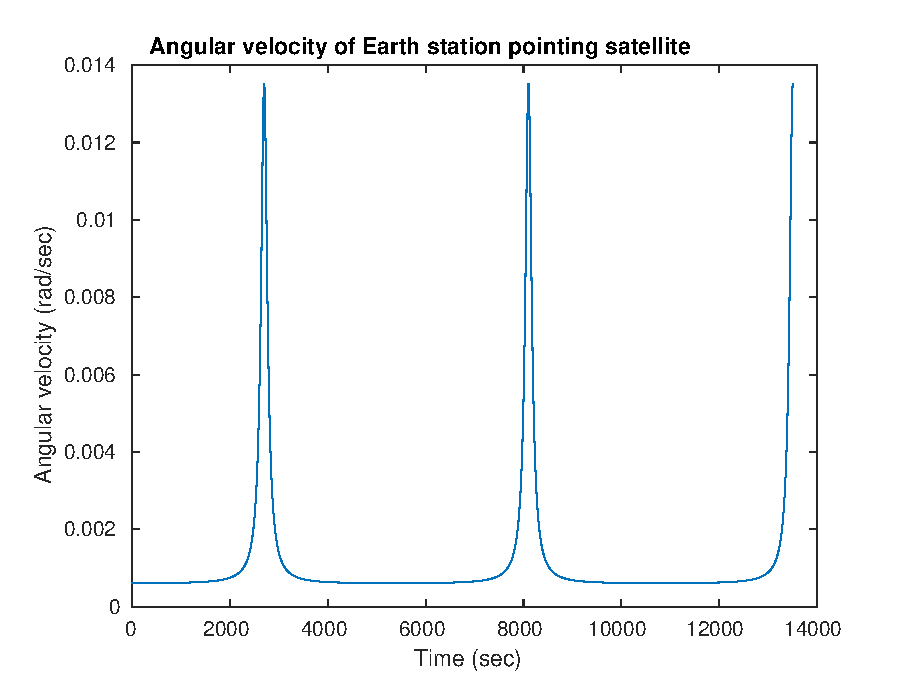
\includegraphics[width=80mm]{figures/maxOmega}
		\caption{Angular Velocity of Earth station pointing satellites.}
		\label{fig:maxOmega}
	\end{subfigure}
	\begin{subfigure}{0.5\linewidth}
	\centering
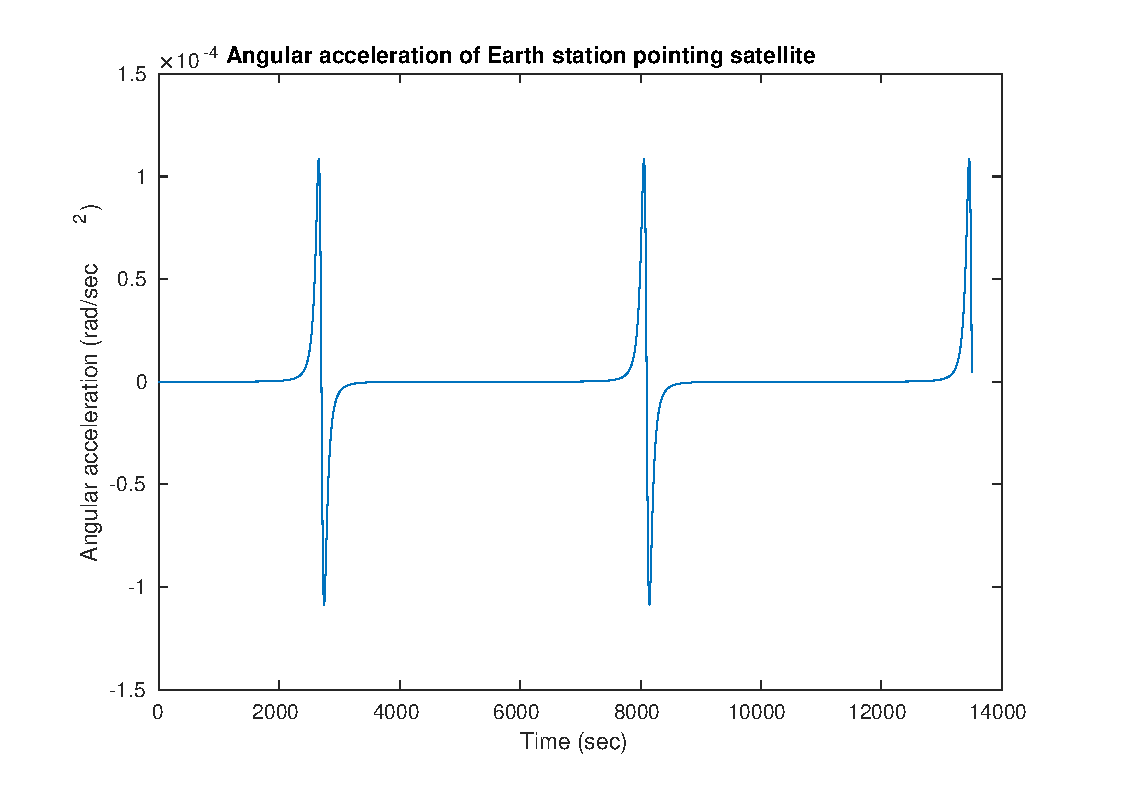
\includegraphics[width=80mm]{figures/maxOmegaDot}
\caption{Angular Acceleration of Earth station pointing satellites.}
\label{fig:maxOmegaDot}
\end{subfigure}
\end{figure} 
